\subsection{AlexNet}
Developped in 2012 by \textcite{krizhevsky_imagenet_2012}, it has won the ImageNet competition. It has made a major breakthrought in the deep \acrshort{cnn} field. It is made of 5 convolutional layers and 3 fully-connected layers. We can see the network on figure \ref{fig:alexnet}.
%
\begin{figure}
    \centering
    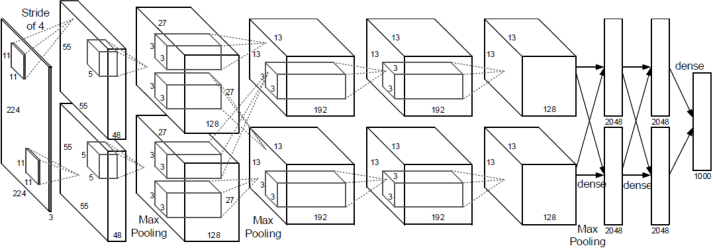
\includegraphics[width=\textwidth]{alexnet.pdf}
    \caption{An illustration of the architecture of AlexNet \cite{krizhevsky_imagenet_2012}}
    \label{fig:alexnet}
\end{figure}
%
\subsection{VGG16}
After the success of AlexNet, research has been made to have a network with same accuracy but lower computational complexity. VGG16 has been introduced by \textcite{simonyan_very_2015} in 2014, which is a deeper variant of AlexNet. It has won the localisation and the second place tracks in ImageNet challenge in 2014. An illustration can be found in figure \ref{fig:vgg}. This depth has been possible by using very small ($3 \times 3$) convolution filters: it allows a large receptive field while having less parameters and more non-linearities than a more larger one. However, it has a high memory request. We need 100MB per image to be stored in all \acrshort{fm}s for the forward propagation
%
\begin{figure}
    \centering
    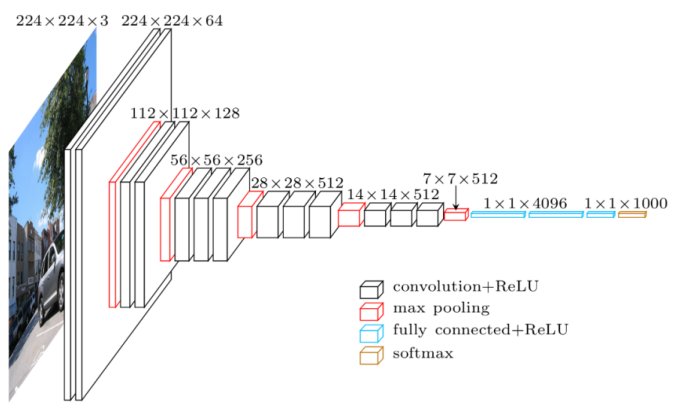
\includegraphics[width=\textwidth]{VGG.pdf}
    \caption{An illustration of the architecture of VGG16 \cite{simonyan_very_2015}}
    \label{fig:vgg}
\end{figure}
%
\subsection{ResNet}
It is a very deep network (152 layers) proposed by \textcite{he_deep_2015}. They have shown that an increase of the depth does not mean an improvement of the performance of the network and this is not due to overfitting. It is because deeper model are harder to optimize dans shallower one (vanishing gradient). But intuitivelly, deeper network should have at least similar or better performance than shallower models. It is explained by the fact that we can map a deeper model into a shallower one by setting the weights to the identity.

Their solution is to add an "identify shortcut connection" that skips one or more layers to mitigate the gradient descent problem and try to set the weights to the identity. We can see the process on figure \ref{fig:resnet}. Weights between the skip connection can be used to learn a residual $F(x)$ to improve the solution. The performance of ResNet allows him to be the 2015 ILSVR winner for both localization and classification.
%
\begin{figure}
    \centering
    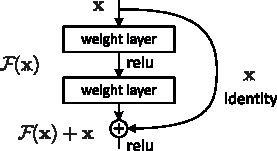
\includegraphics[width=\textwidth]{resnet.pdf}
    \caption{ResNet building block \cite{he_deep_2015}}
    \label{fig:resnet}
\end{figure}
%
\subsection{MobileNetV2}
The drive of the previous networks for accuracy has come for a high computational cost beyond de capabilities of many mobile and embedded applications, according to \textcite{sandler_mobilenetv2_2019}. They have proposed a network tailored for such constrained environment. To do so, we must reduce the size and the number of operations. They have achieved it using \acrshort{dsc}, introduced in section \ref{subs:dsc} and a new layer: inverted residual with linear bottleneck (observed at figure \ref{fig:invreslinbot}). It is first composed of a $1 \times 1$ convolution to expand the number of the input \acrshort{fm} channels and then followed by a \acrshort{dsc}. The intermediate increase of channel is supposed to counterballance the loss of information occured by the ReLU. They have also added a skip connection to build a network of great depth, and the last convolution has a linear activation function.
%
\begin{figure}
    \centering
    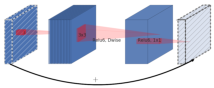
\includegraphics[width=\textwidth]{mbnv2.pdf}
    \caption{inverted residual with linear bottleneck \cite{sandler_mobilenetv2_2019}}
    \label{fig:invreslinbot}
\end{figure}
